\documentclass[border=4pt]{standalone}
\usepackage{fontspec}
\setmainfont{Times New Roman}
\setmonofont{Consolas}
\usepackage{tikz}
\usetikzlibrary{arrows.meta,positioning,shapes.geometric,calc}
\definecolor{tutorteal}{HTML}{087F7A}
\definecolor{tutorlight}{HTML}{EDF7F5}
\definecolor{tutorink}{HTML}{20323C}
\newcommand{\code}[1]{\texttt{\detokenize{#1}}}
\tikzset{box/.style={draw=tutorteal,rounded corners=2pt,fill=tutorlight,
 align=center,minimum height=10mm,text width=35mm,font=\small,inner sep=5pt},
 decision/.style={diamond,aspect=2.0,draw=tutorteal,fill=white,align=center,
 text width=23mm,font=\small,inner sep=1pt},
 flow/.style={-{Latex[length=2mm]},thick,draw=tutorink},
 optional/.style={flow,dashed}}
\begin{document}
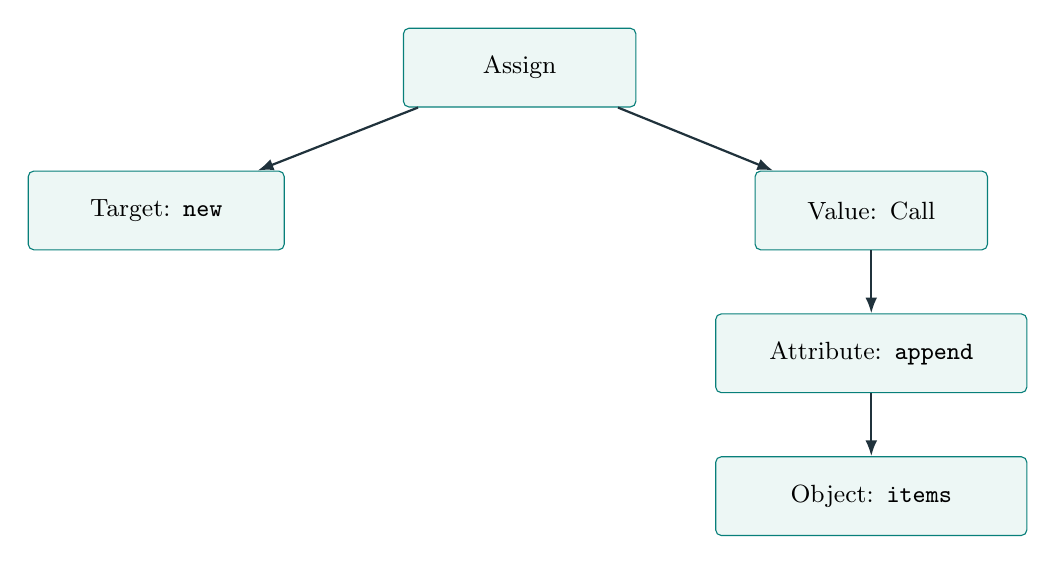
\begin{tikzpicture}[node distance=8mm and 15mm]
\node[box,text width=26mm] (assign) {Assign};
\node[box,text width=29mm,below left=of assign] (target) {Target: \code{new}};
\node[box,text width=26mm,below right=of assign] (call) {Value: Call};
\node[box,text width=36mm,below=of call] (attr) {Attribute: \code{append}};
\node[box,text width=36mm,below=of attr] (obj) {Object: \code{items}};
\draw[flow] (assign)--(target);
\draw[flow] (assign)--(call);
\draw[flow] (call)--(attr);
\draw[flow] (attr)--(obj);
\end{tikzpicture}
\end{document}
